\documentclass[preprint,12pt,reqno]{elsarticle}
\usepackage[left=2cm, right=5cm, top=2cm]{geometry}
\usepackage{graphicx}
\usepackage{amssymb}
\usepackage{amsfonts}
\usepackage{amsthm}
\newtheorem{theorem}{Theorem}
\newtheorem{lemma}[theorem]{Lemma}
\newtheorem{corollary}{Corollary}[theorem]
\newtheorem{definition}{Definition}
\newtheorem{example}{Example}
\usepackage{tikz}
\usepackage{lineno}
\usepackage[english]{babel}
\usepackage{seqsplit}
\usepackage[nottoc]{tocbibind} 
\usepackage[utf8]{inputenc}
\journal{Part C Dissertation Oxford University}
\begin{document}
\begin{frontmatter}
\title{Extensions of number fields with small ramification}
\author{Samuel Bodansky}
\address{Oxford,UK}
\begin{abstract}
Aim: to construct minimally ramified extensions of number fields.
\end{abstract}
\end{frontmatter}
\section{Notation}
\begin{enumerate}
    \item K is a number field, h(K) is its class number and Cl(K) is its ideal class group.
    \item $d_K$ is the discriminant of K.
    \item $K^{ur}$ is the maximally unramified extension of K.
    \item $n_K$ is the degree of the extension $K:\mathbb{Q}$.
    \item KL denotes the compositum of two number fields K and L.
    \item $rd_K$ is the root discriminant of K, $|d_K|^\frac{1}{n_K}$ .
    \item $G_K$ is the Galois group $\Gamma(\bar{K}:K)$
    \item $G_K^{ur}$ is the Galois group $\Gamma(K^{ur}:K)$
    \item $C_K$ is the class field group of K. 
    \item $G^{ab}$ is the abelianisation of a group G, $G/[G,G]$
    \item $K_n$ is the $n_{th}$ term in the sequence defined by $K_0:=K$ and $K_{n+1}$ is the Hilbert class field of $K_n$.
    \item $K_H=\bigcup_{i}K_{i}$ is the Hilbert tower of K.  
    \item $\zeta_n$ is the $n_{th}$ root of unity. 
\end{enumerate}
\section{Summary of Relevant Literature}
\subsection{Jones and Roberts}

\section{Initial Results}
\subsection{Class Field Theory}

Recall a prime ideal $\mathfrak{p}$ in $\mathcal{O}_K$ factors in an extension L of K as
\newline
$\mathfrak{p}\mathcal{O}_L=\mathfrak{B}_1^{e_1}...\mathfrak{B}_m^{e_m}$, where $\mathfrak{B}_i$ are ideals in $\mathcal{O}_L$ intersecting $\mathcal{O}_K$ at $\mathfrak{p}$. Each $e_i\geq1$ and if $e_i>1$ for some i then we say that $\mathfrak{p}$ ramifies in L. If $e_i=1$ for all i then we say $\mathfrak{p}$ splits in L.
\newline
It will also be useful to define the inertia group.\begin{definition}
 Suppose L is an extension of K with Galois group G, $\mathfrak{p}$ is a prime ideal in $\mathcal{O}_K$ and $\mathfrak{B}$ lies above $\mathfrak{p}$ in $\mathcal{O}_L$. Let D be the stabiliser of $\mathfrak{B}$ in G. In addition suppose $\sigma \in D$. Then $\sigma$ induces a map \begin{equation}
     \phi :D\longrightarrow\Gamma(\mathbb{F}_\mathfrak{B}/\mathbb{F}_\mathfrak{p}).
 \end{equation}
 Define the \textbf{Inertia Group}, I, to be the kernel of $\phi$.
\end{definition}
When L is a Galois extension of K, all of the $e_i$ are equal and in fact split(L:K) determines L.
\newline
In fact, if the set of primes that split in L and $\tilde{L}$ then algebraic number theory can show that
\begin{equation}
 split(L:K)=split(L\tilde{L}:K)=split(\tilde{L}:K)
\end{equation}
 and indeed 
 \begin{equation}
 [L:K]=[L\tilde{L}:K]=[\tilde{L}:K].
 \end{equation}
 The following lemma is a useful result in class field theory:
 \begin{lemma}[Abhyankar's Lemma]
    Suppose F is a local field, and $E_1$ and $E_2$ are finite extensions of F with degrees $e_1$ and $e_2$ respectively. In addition, suppose $E_2$ is tamely ramified and $e_2|e_1$. Then $E_1E_2$ is an unramified extension of $E_1$.
 \end{lemma}
A natural question is to determine these sets split(L:K) as L changes over the finite extensions of K, and to determine the sets L corresponding to these extensions.
\newline
Let H be a subgroup of the class group C of K. A finite unramified abelian extension L of K is said to be a $\textit{class field}$ for H if the prime ideals of K splitting in L are exactly those in $\tilde{H}$ . The following theorem provides an answer the above question for unramified abelian extensions of K.
\begin{theorem}
Theorem: A class field exists for each subgroup of C; it is unique, and every finite unramified abelian extension of K is the class group of some subgroup of C. If L is the class field of H, then $\Gamma(L/K)\cong C/H$ and for every prime ideal $\mathfrak{p}$ of K, $f(\mathfrak{p})$ is the order of the image of $\mathfrak{p}$ in the group C/H.
\end{theorem}
We also have this theorem which allows us to define the maximal unramified extension of a number field. 
\begin{theorem}
The composite of two finite unramified extensions of K is also unramified, and so the union $K^{ur}$ of all unramified extensions is also an unramified extension of K. The residue field $\tilde{k}$ of $K^{ur}$ is an algebraic closure of the residue field k of K.
\end{theorem}
\subsection{Hilbert Class Field}
The class field of the trivial subgroup of C is called the Hilbert class field of K. It is maximal abelian extension, L of K unramified at all primes of K.
\newline
For example,if $K=\mathbb{Q}[\sqrt{-5}]$ then take $L=\mathbb{Q}[\sqrt{-1},\sqrt{-5}]$. L is an unramified degree 2 extension of K and so the Hilbert class field of K is $K[\sqrt{-1}]$. Here is a theorem which gives an application of the Hilbert Class Field to Diophantine equations.
\newline

\begin{theorem}
Theorem: Let L be the Hilbert class field of $K=\mathbb{Q}(\sqrt{-n})$, where n is squarefree, $n\not\equiv 3(4)$, so that
\begin{equation}
    \mathcal{O}_K=\mathbb{Z}(\sqrt{-n})
\end{equation}
Assume that p is an odd prime not dividing n, and that x,y are integers. Then 
$p=x^2+ny^2 \Longleftrightarrow$ p splits completely in L.
\end{theorem}
\begin{lemma}
Let L be the Hilbert Class field of K, and let $\mathfrak{p}$ be a prime ideal of K. Then \newline $\mathfrak{p}$ splits completely in L $\Longleftrightarrow\:\mathfrak{p}$ is a principal ideal.
\end{lemma}
\begin{proof}[Proof of Lemma]
We know that $\mathfrak{p}$ splits completely in L iff $(L/K)/\mathfrak{p}=1$. The Artin map induces an isomorphism $C(\mathcal{O}_K)\cong\Gamma(L/K)$. Therefore $(L/K)/\mathfrak{p}=1$ iff $\mathfrak{p}$ determines the trivial class of $C(\mathcal{O}_K)$. But the definition of the ideal class group shows that $\mathfrak{p}$ is principal as required.
\end{proof}
\begin{lemma}
Let L be the Hilbert class field of an imaginary quadratic number field K, and let $\tau$ denote complex conjugation. Then $\tau(L)=L$ whence L is Galois over $\mathbb{Q}$.
\end{lemma}
\begin{proof}
We have the following equivalences:
\begin{equation}
    p=x^2+ny^2\Longleftrightarrow\mathfrak{p}\tmathcal{O}_K=\mathfrak{p}\bar{\mathfrak{p}}; \mathfrak{p}\neq\bar{\mathfrak{p}}; \mathfrak{p}\: principal\:in\: \tmathcal{O}_K
\end{equation}
\begin{equation}
    \Longleftrightarrow\mathfrak{p}\tmathcal{O}_K=\mathfrak{p}\bar{\mathfrak{p}}; \mathfrak{p}\neq\bar{\mathfrak{p}}; \mathfrak{p}\:splits\:completely\:in\:L
\end{equation}
\begin{equation}
    \Longleftrightarrow\:p\:splits\:completely\:in\:L.
\end{equation}
The first equivalence comes from the factorisation 
\begin{equation}
    p=x^2+ny^2=(x+\sqrt{-ny})(x+\sqrt{ny}).
\end{equation}
The second and third equivalences come from the above two lemmas respectively.
\end{proof}
\begin{corollary}
Suppose $K=\mathbb{Q}{\sqrt{-n}}$ n is positive,squarefree, $n\not\equiv 3(4)$, so that $d_K=-4n$. If p is an odd prime not dividing n, then
\begin{equation} p=x^2+ny^2 \Longleftrightarrow p\:splits\:completely\:in\:the\:Hilbert\:class\:field\:of\:K.
\end{equation}
Hence the primes of the form $x^2+ny^2$ characterise the Hilbert Class field of $\mathbb{Q}(\sqrt{-n})$.
\end{corollary}
In fact Bruckner \cite{BRUC} generalises this theorem when L is a \textit{generalised dihedral} extension of K over $\mathbb{Q}$. Suppose K is an imaginary quadratic field and L is an abelian extension of K which is Galois over $\mathbb{Q}$; let $\tau$ represent complex conjugation. Write
\begin{equation}
   \Gamma(L/\mathbb{Q})\cong \Gamma(L/K)\rtimes(\mathbb{Z}/2\mathbb{Z})
\end{equation}
where the non-identity element of $\mathbb{Z}/2\mathbb{Z}$ acts on $\Gamma(L/K)$ via conjugation with $\tau$.
\begin{definition}
 We say L is \textbf{generalised dihedral} over $\mathbb{Q}$ if this action acts as the inverse map on $\Gamma(L/K)$.
\end{definition}

\begin{theorem}
Let K be an imaginary class field. Then an abelian extension L of K is generalised dihedral over $\mathbb{Q}$ iff L is contained in a ring class field of K.
\end{theorem}
\section{Infinite Unramified Extensions}
Suppose K is a class field with trivial class group, i.e. h(K)=1. Then K has no abelian (and hence no
solvable) non-trivial unramified Galois extension. Despite this, K may have a non-solvable unramified extension. \cite{BRIN} gives such an example. Suppose
\begin{equation}
   K=\mathbb{Q}(\sqrt{29},\sqrt{4967}) 
\end{equation}
\begin{equation}
   L=split(x^7 - 11x^5 + 17x^3 - 5x + 1,\mathbb{Q}[x])
\end{equation}
Then K has class number 1 and L is a PSL(2, 7)-extension of K.
\cite{MAIR} showed that there exist biquadratic number fields with class number one with an infinite unramified extension. 
\begin{theorem}
\cite{BRIN} Suppose that \begin{enumerate}
    \item $f\in \mathbb{Z}[x]$ is an irreducible quintic with five real roots
    \item $D=\Delta(f)$ is prime and $\mathbb{Q}(\sqrt{L})$ has class number 1
    \item p and q are two primes such that $\mathbb{Q}(\sqrt{p.q})$ has class number 1 and $\mathbb{Q}(\sqrt{(D.p.q})$ has class number 2.
    \item f has five simple roots modulo p and f factors modulo q into polynomials of degrees, as a tuple $\mu$ of the form (1,1,1,1,1),(1,1,1,3),(1,2,2) or (1,1,3).
\end{enumerate}
Then the field $L=\mathbb{Q}(\sqrt{D},\sqrt{p.q})$ has class number 1 and infinite unramified extension.
\end{theorem}
\begin{proof}
A result from \cite{KOND} shows that the splitting field K
of f is an $S_5$-extension of $\mathbb{Q}$ and an unramified $A_5$-extension of $\mathbb{Q}(\sqrt{D})$. Hence $M=K(\sqrt{p.q})$ is an
unramified $A_5$-extension of L. Furthermore, K has class number 1, as demonstrated in the following diagram.
\begin{center}
    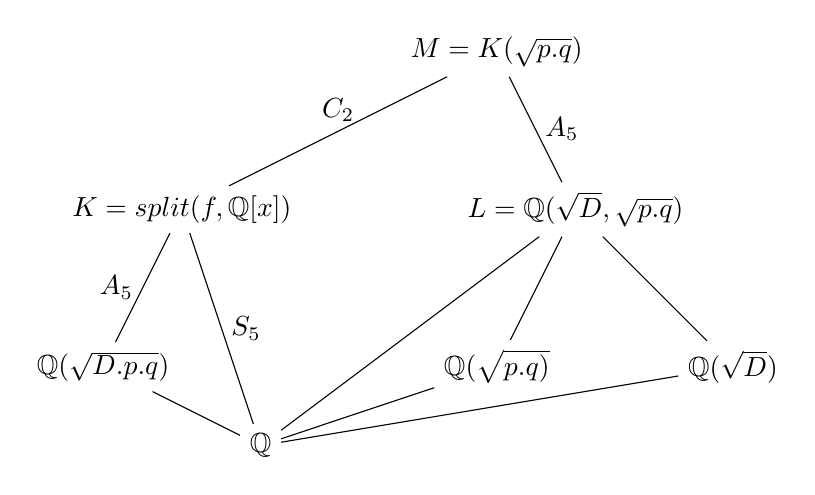
\begin{tikzpicture} [align=center]
  \path  (0, 0)   node(Q)  {$\mathbb{Q}$}
          +(6, 1)   node(QD) {$\mathbb{Q}(\sqrt{D})$}
          ++(3,1)   node(Q12) {$\mathbb{Q}(\sqrt{p.q)}$}
           ++(-5,0)   node(QD12) {$\mathbb{Q}(\sqrt{D.p.q})$}
           ++(1,2)   node(K) {$K=split(f,\mathbb{Q}[x])$}
           ++(5,0)   node(L) {$L=\mathbb{Q}(\sqrt{D},\sqrt{p.q})$}
            ++(-1,2)   node(M) {$M=K(\sqrt{p.q})$};
    \draw [-] (Q) to node [pos=0.5,above]{} (Q12);
    \draw [-] (Q) to node [pos=0.8,below]{} (QD12);
    \draw [-] (Q) to node [pos=0.5,below]{} (QD);
  \draw [-] (QD12) to node [pos=0.5,left]{$A_5$} (K);
  \draw [-] (Q) to node [pos=0.5,right]{$S_5$} (K);
  \draw [-] (Q) to node [pos=0.5,below]{} (L);
  \draw [-] (Q12) to node [pos=0.5,below]{} (L);
  \draw [-] (QD) to node [pos=0.5,below]{} (L);
    \draw [-] (L) to node [pos=0.5,right]{$A_5$} (M);
     \draw [-] (K) to node [pos=0.5,above]{$C_2$} (M);
\end{tikzpicture}
\end{center}

Let r be the number of primes $\mathfrak{p}$ in L ramified in M, and let $\theta$ be a root of f, $T = \mathbb{Q}(\theta)$. \cite{MAR1} shows that M has an infinite 2-class field tower if $r\geq 155$. By assumption p splits completely in T and therefore also in L; furthermore q decomposes in T as $q = \mathfrak{p}_1...\mathfrak{p}_r$, with inertia degrees
\begin{equation}
    (deg(\mathfrak{p}_1),...deg(\mathfrak{p}_r))=\mu 
\end{equation}
Write $Z_\mathfrak{B}\subseteq\Gamma(L/\mathbb{Q}) = S_5$; as the decomposition group of $\mathfrak{B}$ where $\mathfrak{B}$ is a prime in L dividing q. q is unramified so this group is cyclic, and \cite{ART1} shows that $Z_\mathfrak{B}$ has order at most 3.  It now follows that L has 120 primes dividing p and at least 40 primes dividing q. Then $r\geq 160$ since they all ramify in M, and the theorem follows.
\end{proof}
There are 9 imaginary quadratic fields with class number 1 and 47 imaginary biquadratic number fields with class number 1. Odlyzko's bound (even not assuming GRH) show that no imaginary quadratic number field with trivial class group has an infinite unramified extension. Such a method does not work for imaginary biquadratic number fields with trivial class group, by considering the field $K=\mathbb{Q}(\sqrt{-67},\sqrt{-163})$ which has root discriminant approximately 104.5.

Using SageMath, the following polynomial and primes were found:
\begin{equation}
    f(x)=x^5+4x^4-6x^2-x+1, p=1531,q=71,151,227,\Delta(f)=170701
\end{equation}
\begin{equation}
 f(x)=x^5-4x^4+12x^2-8x+1,p=1987,q=31,107,211,239,\Delta(f)=186037
 \end{equation}
These satisfy the criteria of the above theorem and therefore describe field with infinite unramified extension. 
%[1,-1,-6,0,4,1],1531, 71, 'for sure
\subsection{First results}
Goal: For a given number field K, what is the maximal unramified extension $K^{ur}$ of K is and also what is the structure of $G_K^{ur}$ is. By Class Field Theory we already know that 
\begin{equation}
  (G_K^{ur})^{ab} = \Gamma(K_1:K)\cong C_K
\end{equation}

\subsection{Important Results from Class Field Theory}
1. \cite{YAMA}[Proposition 1] gives the following classification of polynomials of the form $f(x) = x^n+ax+b \in \mathbb{Z}[x]$, and K is the splitting field of f over $\mathbb{Q}$.
\newline
If the following conditions hold:
\begin{enumerate}
    \item (n-1)a and nb are relatively prime 
    \item $\Gamma(K/\mathbb{Q}) \cong S_n$
\end{enumerate}
\newline
Then K is an $A_n$-extension of $\mathbb{Q}(\sqrt{\Delta(f)})$ which is unramified at all finite primes. For example, if $f(x) = x^5-x+1$, then $\Delta(f)= 2869$ and write $L = \mathhbb{Q}(\sqrt{2869})$. Then K is unramified over L and $\Gamma(K:L)\cong A_5.$

\section{Bounds on Discriminants}
Minkowski's theorem bound shows that if K is a number field with $r_1$ real and $2*r_2$ complex conjugate fields, and $n=r_1+2r_2$ is the degree of the field, then 
\begin{equation}
rd_K\geqslant (\frac{\pi}{4})^{\frac{2r_1}{n}}\frac{n^2}{n!^{\frac{2}{n}}}
\end{equation} 
As $n\rightarrow \infty$, Stirling's formula can give a bound that
\begin{equation}
    rd_K\geqslant e^2 = 7.39
\end{equation}
Odlyzko's Bound \cite{ODL2} improved on the bounds for Minkowski for the discriminant of a number field. It can be stated as  
\begin{equation}
rd_K\geqslant 60^{\frac{r_1}{n}}22^{\frac{r_2}{n}}+o(1)\:as\:n\rightarrow \infty   
\end{equation}
Furthermore, under the assumption of the Generalised Riemann Hypothesis, 
this bound can be improved by replacing the numbers 60 and 22 by 188 and 41 respectively. 
\subsection{How to use this bound}
Following \cite{YAMA}, write this bound function as $B(n,r_1,r_2)$.
\begin{theorem}
Suppose that H is a positive integer, and L is an unramified normal extension of K of degree M. Then if
\begin{enumerate}
    \item If \begin{equation}
        rd_K<B(H.m.n,H.m.r_1,H.m.r_2)
    \end{equation}
    then $[K^{ur}:L]<H$ and $h(L)<H$. Indeed if H=2 then $K^{ur}=L$.

    \item If
        $h(L)=1$ and H=60 then again $K^{ur}=L$.
\end{enumerate}
\end{theorem}
\subsection{Result using Hoelscher}

Using \cite{HOEL} and \cite{JONE}, we see that 
the prime p=239 is tamely ramified for 
\begin{equation}
  G=S_3,G\textsuperscript{ab} = 2, p_w =3  
\end{equation} and also 
\begin{equation}
    G=D_5,G\textsuperscript{ab} = 2 
\end{equation}
This means that we can apply Theorem(1.1) from Hoelscher with
\begin{equation}
    N = G = D_5, K_0 = \mathbb{Q}
\end{equation}
Then 
\begin{equation}
N/p(N) = D_5 \not\subset \mathbb{Z}/(p-1) = \mathbb{Z}_{238}
\end{equation}
\newline
We have the field extension diagram
\bigskip
\newline
\begin{center}
    
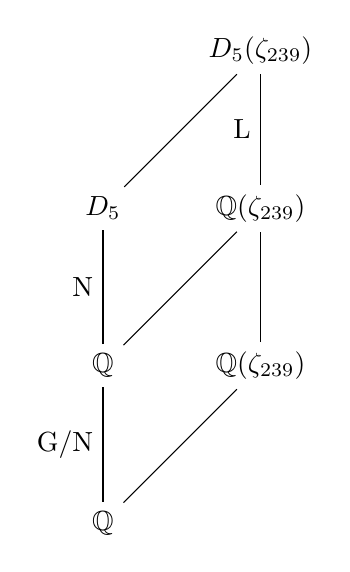
\begin{tikzpicture}[node distance = 2cm, auto]
      \node (Q) {$\mathbb{Q}$};
      \node (K0) [above of=Q] {$\mathbb{Q}$};
       \node (QZP) [above of=Q, right of=Q] {$\mathbb{Q}(\zeta_{239})$};
       \node (K) [above of=K0] {$D_5$};
       \node (K0ZP) [above of=QZP] {$\mathbb{Q}(\zeta_{239})$};
       \node (KZP) [above of=K0ZP] {$D_5(\zeta_{239})$};
       
       \draw[-] (Q) to node {G/N} (K0);
       \draw[-] (K0) to node {N} (K);
       \draw[-] (K) to node {} (KZP);
       \draw[-] (K0ZP) to node {L} (KZP);
       \draw[-] (QZP) to node {} (K0ZP);
       \draw[-] (Q) to node {} (QZP);
       \draw[-] (K0) to node {} (K0ZP);
      \end{tikzpicture}
\end{center}
\newline
Where the field extension L is a non-trivial abelian unrafimifed sub-extension of degree prime to p with L Galois over $\mathbb{Q}$.
\subsection{Maire's Results for infinite non Galois unramified extension}
Following from \cite{MAIR}[5.1], there exist infinitely many quadratic fields with a finite 2-Hilbert tower, but having an infinite ramified extension of $2^{\infty{}}$. 
The following methodology was implemented  to find suitable polynomials:
\newline
\begin{enumerate}
    \item Pick 8 real numbers close to 0 and define $\tilde{P}(x)$ to be the polynomial with these roots. This is done to increase the probability that P(x) will also have 8 real roots. 
    \item Find a polynomial P(x) which is near to $\tilde{P}(x)$.
    \item Check that the P(x) is irreducible, has 8 real roots and has prime discriminant. 
    \item Search for primes 3 mod 4 which totally decompose in the splitting field of P. 
\end{enumerate}
The following polynomial was found: 
\begin{equation}
    P(X) = (x^8 - 3x^7 - 16x^6 + 31x^5 + 74x^4 - 40x^3 - 56x^2 + 17x + 3)
\end{equation}
where 
\begin{equation}
    l = \Delta(P) = 76363470193820546413
\end{equation}
Put \begin{equation}
    q_1 = 219823, q_2 = 931363, K = split(P, \mathbb{Q}[x]).
\end{equation}
\newline
Here $q_1$ and  $q_2$ are totally decomposed in $K/\mathbb{Q}$, the Galois closure of P.
\newline
Use the following definitions: 
\begin{itemize}
    \item $N = K\mathbb{Q}(\sqrt{l})$. Note $q_1$ and $q_2$ decompose completely in $N/\mathbb{Q}$, an extension of degree 16.
    \item $E = N(\sqrt{q_1.q_2})$
    \item $E_2$ is the infinite 2-Hilbert tower of E.
\end{itemize}
\newline 
We can now draw the following field diagram, where all extensions are unramified 2-extensions. 

\begin{center}
    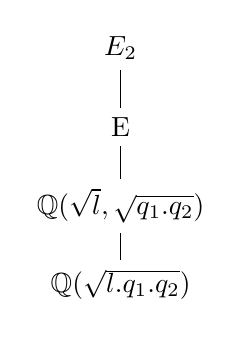
\begin{tikzpicture}[node distance = 1cm, auto]
      \node (Q12) {$\mathbb{Q}(\sqrt{l.q_1.q_2})$};
      \node (QL12) [above of=Q12] {$\mathbb{Q}(\sqrt{l},\sqrt{q_1.q_2})$};
      \node (E) [above of=QL12] {E};
      \node (E2) [above of=E] {$E_2$};
      \draw [-] (Q12) to node {} (QL12);
      \draw [-] (QL12) to node {} (E);
      \draw [-] (E) to node {} (E2);
      \end{tikzpicture}
\end{center}
\newline
In fact, $E_2/\mathbb{Q}(\sqrt{l.q_1.q_2})$ is an unramified field extension of degree $2^{\infty}$.
\section{Kim and Koenig}
\begin{theorem}
 Define $K=\mathbb{Q}(\sqrt{22268})$, $L=split(x^6-10x^4-7x^3+15x^2+14x+3,\mathbb{Q}[x])$. Then $K_1=\mathbb{Q}(\sqrt{76},\sqrt{293})$. Define $M=LK_1$. Then $M=K^{ur}$ and we have the following diagram.   
\end{theorem}
\begin{center}
    \begin{tikzpicture}[node distance = 1.8cm, auto]
      \node (Q) {$\mathbb{Q}$};
      \node (K) [above of=Q] {K};
      \node (K1) [above of=K] {$K_1$};
      \node (M) [above of=K1] {$M=LK_1$};
      \node (L) [right of=K1] {L};
    \draw [->,out=180,in=180,looseness=1] (Q.west) to node[above][pos=0.6,left]{$A_5\times V_4$}  (M.west);    
    \draw [-] (Q) to node [pos=0.1,left]{$C_2$} (K);
    \draw [-] (K) to node {} (K1);
    \draw [-] (K1) to node {$A_5$} (M);
    \draw [-] (Q) to node [pos=0.6,right]{$A_5$} (L);
    \draw [-] (L) to node [pos=0.1,right,above]{$V_4$} (M);
      \end{tikzpicture}
\end{center}
Now define $K=\mathbb{Q}(\sqrt{-1567})$ and 
\begin{equation}
    L=split(x^9-2x^8+10x^7-25x^6+34x^5-40x^4+52x^3-45x^2+20x-4,\mathbb{Q}[x])
\end{equation}Then we use the following theorem
\begin{theorem}
    Write $G=PSL_2(\mathbb{F}_8)$. L is a G-extension of $\mathbb{Q}$; 1567 is the only prime in this field which is ramified with index 2. Abhyankar's Lemma shows that LK/K is unramified at every prime. G is a nonabelian simple group and so $L\capK_1=\mathbb{Q}$. Therefore $\Gamma(LK_1/K_1)\cong\Gamma(L/\mathbb{Q})\cong G$. It follows that $\Gamma(LK_1/\mathbb{Q})\cong G\times D_{15}$.
\end{theorem}
We have the following diagram:
\begin{center}
    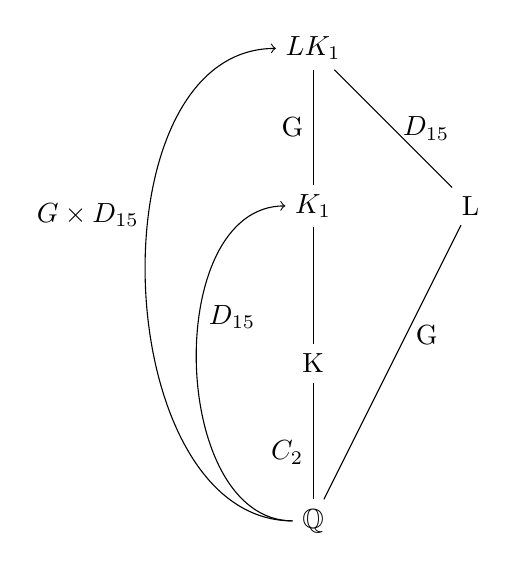
\begin{tikzpicture}[node distance = 2cm, auto]
      \node (Q) {$\mathbb{Q}$};
      \node (K) [above of=Q] {K};
      \node (K1) [above of=K] {$K_1$};
      \node (LK1) [above of=K1] {$LK_1$};
      \node (L) [right of=K1] {L};
    \draw [->,out=180,in=180,looseness=1] (Q.west) to node[above][pos=0.6,left]{$G\times D_{15}$}  (LK1.west);
    \draw [->,out=180,in=180,looseness=1] (Q.west) to node[above][pos=0.6,right]{$D_{15}$}  (K1.west); 
    \draw [-] (Q) to node [pos=0.4,left]{$C_2$} (K);
    \draw [-] (Q) to node [pos=0.6,right]{G} (L);
    \draw [-] (K) to node {} (K1);
    \draw [-] (K1) to node {G} (LK1);
    \draw [-] (L) to node [pos=0.5,right]{$D_{15}$} (LK1);
      \end{tikzpicture}
\end{center}
\section{Yamamura's Results}
\cite{YAM2} $\mathbb{Q}(\sqrt{-1507})$ is the first imaginary quadratic field with an unramified $A_5$-extension over $\mathbb{Q}$. In fact, defining $L=split(x^5-5x^3+5x^2+24x+5,\mathbb{Q}[x])$ gives such an $A_5$ extension of K. 
\begin{lemma}
Define $K=\mathbb{Q}(\sqrt{-14731})$, $L=split(x^6+3x^5,5x^4+4x^3+3x^2+2x+1,\mathbb{Q}[x])$. Then L is an unramified $A_6$-extension of K and is an $S_6$ extension of $\mathbb{Q}$.
\end{lemma}
\begin{lemma}
Define $K=\mathbb{Q}(\sqrt{-30759})$, $L=split(x^7+2x^6-3x^4-x^3-x^2-x+2,\mathbb{Q}[x])$. Then L is an unramified PSL(2,7)-extension of K and is an $PSL(2,7)\times C_2$ extension of $\mathbb{Q}$.
\end{lemma}
\section{Trying to recreate Maire's Results}
In \cite{MAIR}[3.1] I use Maire's method to find a suitable polynomial.
Firstly, we invoke the following theorem:
\begin{theorem}[Kummer Theory]
Suppose $K/\mathbb{Q}$ is a cyclic extension of degree p,unramified at p, and $L/\mathbb{Q}$ is an extension of degree n. Suppose also that for all places $\mathfrak{Q}$ in L, the ramification index of $\mathfrak{Q}$ in $L/\mathbb{Q}$ divides the ramification index of $\mathfrak{q} = \mathbb{Q}\cap\mathfrak{Q}$ in $K/\mathbb{Q}$. \newline
Then the extension $LK/\mathbb{Q}$ is unramified at all finite places. In particular, $\bar{L}K/K$ is also unramified at all finite places.
\end{theorem}
Using SageMath, the following polynomial and primes were found. Define 
\begin{equation}
    P(x) = x^7-3x^6-5x^5+17x^4+x^3-14x^2+3x+1, l=\Delta(P)=8980833629
\end{equation}
Also define $K=split(P,\mathbb{Q}[x])$. Modulo l,
\begin{eqnarray*}
        P(x)&=&(x+2040911047)(x+3097257563)\\ & & {} (x+3210721157)(x+6041496066)\\ & & {}(x+6737752038)(x+7397598321)^2
\end{eqnarray*}
Now specify values for $q_1$ and $q_2$:
\begin{equation}
    q_1=17471,q_2\in\{443,919,1627,2803,3691,5231,5867,9391\}
\end{equation}
Then indeed $q_1\equiv\:q_2\equiv3(4)$.$q_1$ splits completely in K, there are n-1 places lying above $q_2$ in $K/\mathbb{Q}$.
\newline
Define $L=\mathbb{Q}(\sqrt{l.q_1.q_2})$, $M=KL$. Using the above theorem, all places lying above $q_1$ and $q_2$, in addition to n-2 places above l are ramified in M/K.  Applying \cite{MAIR}[Proposition 2.2] shows that M/L is nowhere ramified. Thus we get the following field extensions
\begin{center}
    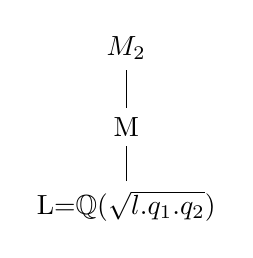
\begin{tikzpicture}[node distance = 1cm, auto]
      \node (L) {L=$\mathbb{Q}(\sqrt{l.q_1.q_2})$};
      \node (M) [above of=L] {M};
      \node (M2) [above of=M] {$M_2$};
      \draw [-] (L) to node {} (M);
      \draw [-] (M) to node {} (M2);
      \end{tikzpicture}
\end{center}
where $M_2/L$ is an infinite unramified extension. We therefore have the following theorem:
\begin{theorem}
    Suppose K is a quadratic field of the form $\mathbb{Q}(\sqrt{8980833629.17471.q_2})$, where 
    \begin{equation}
        q_2\in\{443,919,1627,2803,3691,5231,5867,9391\}
    \end{equation}
    then \begin{enumerate}
        \item $K_H/K$ is finite
        \item $K_\infty/K$ is finite.
    \end{enumerate}
\end{theorem}
\cite{MAIR}[2.1] gives a condition for the p-Hilbert tower of K to be infinite; \cite{MAIR}[2.3] says that if P is an irreducible real polynomial in $\mathbb{Q}[x]$ with squarefree discriminant D(P), and C is its Galois closure, then $C/\mathbb{Q}(\sqrt{\Delta(P)})$ is unramified.
\newline
Using these two propositions from Maire can give an algorithm to find a field $K=\mathbb{Q}(\sqrt{l_1.l_2.l_3)}$, where $l_1$ is a prime 1 modulo 4, and $l_2$ and $l_3$ are primes 3 modulo 4. 
\newline
Here is an example for n= 5:
\begin{equation}
    x^5 + 12x^4 + 20x^3 - 96x^2 - 4399, D=1255760665676742389.
\end{equation}
\section{Kondo's Results}
\begin{theorem}
    Suppose F is a number field with discriminant d(F) of degree n, and K is its Galois closure over $\mathbb{Q}$. Suppose d(F) is not a square, i.e. it is equal to the discriminant of the quadratic number field $\mathbb{Q}(\sqrt{d(F)})$, then \begin{enumerate}
        \item $\Gamma(K:\mathbb{Q})\cong S_n$
        \item $K/\mathbb{Q}(\sqrt{d(F)})$ is an unramified extension.
    \end{enumerate}
\end{theorem}
Furthermore we have the following theorem \begin{theorem}
    The following are equivalent: \begin{enumerate}
        \item d(F) is equal to the discriminant of the quadratic number field $\mathbb{Q}(\sqrt{d(F)})$
        \item For every prime dividing d(F), its ideal $\mathfrak{p}$ in F has precisely one ramified divisor.
    \end{enumerate}
\end{theorem}
\begin{lemma}
Furthermore, the following condition is equivalent to the above:
\newline
    The inertia group of every ramified prime of K is a group of order 2 generated by a transposition.\newline
In particular, if F satisfies the above condition, then d(F) is equal to $\Delta(\mathbb{Q}(\sqrt{d(F)}))$.
\end{lemma}
\begin{proof}
This is immediate from a theoreom of Van der Waerden. 
\end{proof}
\begin{lemma}
Suppose $d(F)\notin \mathbb{Q}^2$. Then the following are equivalent:\begin{enumerate}
    \item K is an unramified extension of $\mathbb{Q}(\sqrt{d(F)})$
    \item The inertia group of every ramified prime of K is a group of order 2,generated by an odd permutation. 
\end{enumerate}
\end{lemma} 
The following examples were found using SageMath
\begin{example}
Define $f(x)=x^6 + x^5 - 6x^4 - 4x^3 + 8x^2 + 3x - 2$. Also define $F=\mathbb{Q}(\theta)$, where $\theta$ is a root of f, and let K be the splitting field of f over $\mathbb{Q}$. Then we get $d(f)=\Delta(F)=7846061=17^3.1597$. \begin{equation}
   f(x)= (x^3 + 9x^2 + 16x + 7)^2\:modulo\:17
\end{equation}
By the above lemmas, we see that K is an unramified extension of $\mathbb{Q}(17^3.1597)$. Furthermore, $\Gamma(K/\mathbb{Q})$ is a group of order 72 and is isomorphic to the wreath product of $S_3$ and $C_2$. It follows that $K/\mathbb{Q}(\sqrt{17^3.1597})$ is an unramified extension with Galois group isomorphic to the Frobenius group of order 36.
\end{example}
\begin{example}
Define $f(x)=x^6 + 2x^5 - 6x^4 - 5x^3 + 6x^2 + 2x - 1$. Also define F and K as above. Then we get $d(f)=\Delta(F)=18295573=257^2.277$. \begin{equation}
   f(x)= (x + 124)^2 (x + 143)^2  (x^2 + 239x + 256)\:modulo\:257
\end{equation}
By the above lemmas, we see that K is an unramified extension of $\mathbb{Q}(257^2.277)$. Furthermore, $\Gamma(K/\mathbb{Q})$ is a group of order 48 and is isomorphic to the wreath product of $C_2$ and $S_3$. It follows that $K/\mathbb{Q}(\sqrt{257^2.277})$ is an unramified extension with Galois group isomorphic to $S_4$. %(Check)
\end{example}
\section{Using Sympy to find Maximal Unramified Extensions}
Here is an algorithm to find the maximal unramified extension of a number field using Odlyzko's bound and result from Kim \& Koenig and Maire.
\begin{enumerate}
  \item  Order the irreducible quintic polynomial in $\mathbb{Z}[x]$ by the absolute value of their discriminant. 
  \item Pick f(x) to be a possible quintic polynomial.
  \item Calculate $\Delta(f(x))$ and check it is squarefree.
  \item Check that f(x) has precisely three real roots. 
  \item Let S be the splitting field of f, and therefore $\Gamma(S:\mathbb{Q})\cong S_5$
  \item Define $K=\mathbb{Q}(\sqrt{\Delta})$ and therefore $\Gamma(S:K)\cong A_5$. Note by Proposition 2.3 in Maire, S is an unramified extension of K. 
  \item Calculate the root discriminant of K, $rd_K$.
  \item Use the Odlyzko bound to calculate the degree of the maximal unramified extension. If we can show that $[K^{ur}:K]<120$ and $[K^{ur}:\mathbb{Q}]<240$ by the Tower Law, then indeed $K^{ur} = S$.
\end{enumerate}
\newline
In fact, we can draw the following diagram: 
\newline
\begin{center}
    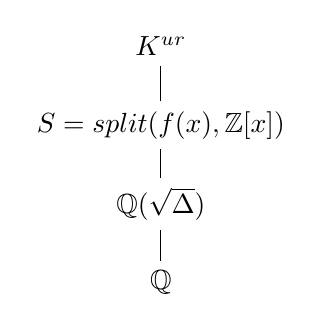
\begin{tikzpicture}[node distance = 1cm, auto]
      \node (Q) {$\mathbb{Q}$};
      \node (K) [above of=Q] {$\mathbb{Q}(\sqrt{\Delta})$};
      \node (S) [above of=K] {$S=split(f(x),\mathbb{Z}[x])$};
      \node (Kur) [above of=S] {$K^{ur}$};
      \draw [-] (K) to node {} (S);
      \draw [-] (Q) to node {} (K);
      \draw [-] (S) to node {} (Kur);
      \end{tikzpicture}
\end{center}
Using Cohn(1955) and verifying with computer search we calculate that a quintic polynomial that satisfies the above conditions, and has minimal absolute discriminant is $f(x) = x^5-2x^3-x^2+1$ which has $\Delta(f) = -4511\equiv1(4)$.
This polynomial has root discriminant = 67.16.
Using the bounds in given in Table(2) of Odlyzko(1990) we find that indeed
\begin{equation}
    K^{ur}\cong A_{5}
\end{equation}
\begin{thebibliography}{9}
\title{References}
\bibitem{HOEL} 
Long Hoelscher, Jing, \textit{Galois extensions ramified at one prime} (2007). Dissertations available from ProQuest. AAI3260949. 
\bibitem{JONE} 
Jones J.W., Roberts D.P. (2008) \textit{Number Fields Ramified at One Prime}. In: van der Poorten A.J., Stein A. (eds) Algorithmic Number Theory. ANTS 2008. Lecture Notes in Computer Science, vol 5011. Springer, Berlin, Heidelberg
\bibitem{KIM1}
Kim, Kwang-Seob. \textit{Construction of unramified extensions with a prescribed Galois group}. Osaka J. Math. 52 (2015), no. 4, 1039--1051. https://projecteuclid.org/euclid.ojm/1447856031
\bibitem{MAIR}
Maire, Christian. (2006). \textit{On infinite unramified extensions. Pacific Journal of Mathematics}. 192. 10.2140/pjm.2000.192.135. 
\bibitem{ODL1}
Odlyzko, A. M. \textit{Bounds for discriminants and related estimates for class numbers, regulators and zeros of zeta functions : a survey of recent results}. Journal de théorie des nombres de Bordeaux, Volume 2 (1990) no. 1, pp. 119-141. 
\bibitem{ODL2}
Odlyzko, A. M. \texit{Lower bounds for discriminants of number fields}, II. Tohoku Math. J. (2) 29 (1977), no. 2, 209--216.  https://projecteuclid.org/euclid.tmj/1178240652
\bibitem{KIM2}
Kim, Kwang-Seob & Koenig, Joachim. (2017). Some examples of quadratic fields with finite nonsolvable maximal unramified extensions II. The Ramanujan Journal. 10.1007/s11139-018-0046-3. 
\bibitem{YAMA}
Yamamoto, Yoshihiko. On unramified Galois extensions of quadratic number fields. Osaka J. Math. 7 (1970), no. 1, 57--76. https://projecteuclid.org/euclid.ojm/1200692686
\bibitem{BRIN}
Brink, David. (2010). Remark on infinite unramified extensions of number fields with class number one. Journal of Number Theory - J NUMBER THEOR. 130. 304-306. 10.1016/j.jnt.2009.08.013. 
\bibitem{DIAZ}
 F. Diaz Y. Diaz, Tables minorant la racine n-ième du discriminant d'un corps de degré n. Publications Mathématiques d'Orsay 80.06. Université de Paris-Sud, Département de Mathématique, Orsay, (1980). 59 pp. MR 82i:12007.
 \bibitem{BRUC}
 G. Bruckner, Charakterisierung der galoisschen Zahlkorper, deren. 2. E. Artin, Galois Theory, University of Notre Dame, Notre Dame, Indiana, 1959.
 \bibitem{KOND}T. Kondo, Algebraic number fields with the discriminant equal to that of a quadratic number field, J. Math. Soc. Japan 47 (1)
(1995) 31–36.
\bibitem{MAR1}
 J. Martinet, Tours de corps de classes et estimations de discriminants, Invent. Math. 44 (1978) 65–73
\bibitem{ART1}
 B.L. van der Waerden, Die Zerlegungs- und Trägheitsgruppe als Permutationsgruppen, Math. Ann. 111 (1935) 731–733
 \bibitem{YAM2}
 Yamamura, Ken. Maximal unramified extensions of imaginary quadratic number fields of small conductors. Journal de théorie des nombres de Bordeaux, Volume 9 (1997) no. 2, pp. 405-448.
 \bibitem{KOND}
 KONDO, Takeshi. Algebraic number fields with the discriminant equal to that of a quadratic number field. J. Math. Soc. Japan 47 (1995), no. 1, 31--36. doi:10.2969/jmsj/04710031.
\end{thebibliography}

\end{document}

